\chapter{Конструкторская часть}

\section{Алгоритмы нахождения редакционного расстояния}


В данной части будут рассмотрены схемы алгоритмов нахождения расстояния Левенштейна и Дамерау-Левенштейна.
На рисунках 2.1-2.4 представлены данные алгоритмы.

\begin{figure}[h]
	\centering
	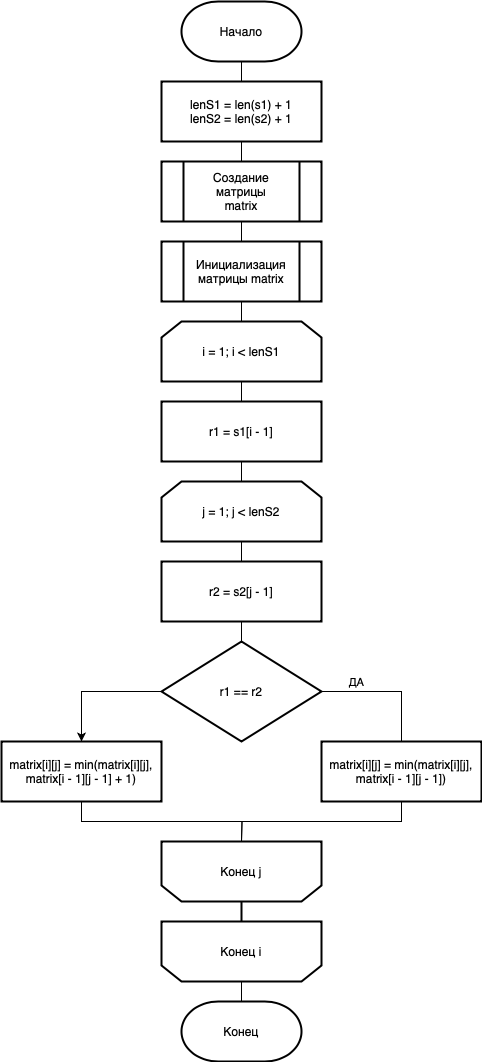
\includegraphics[width=0.46\linewidth]{img/L.png}
	\caption{Схема нерекурсивного алгоритма нахождения расстояния Левенштейна}
	\label{fig:mpr}
\end{figure}

\clearpage

\begin{figure}[h]
	\centering
	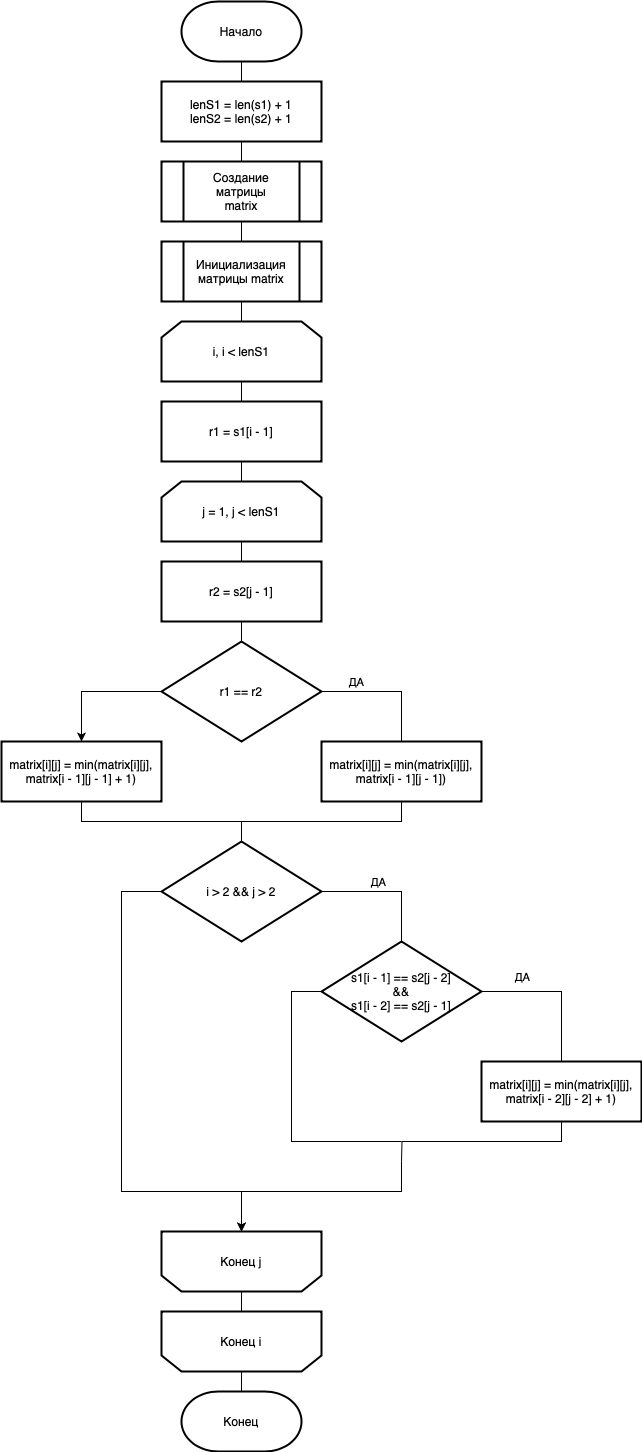
\includegraphics[width=0.65\linewidth]{img/DLM.png}
	\caption{Схема нерекурсивного алгоритма нахождения расстояния Дамерау-Левенштейна}
	\label{fig:mpr}
\end{figure}

\clearpage

\begin{figure}[h]
	\centering
	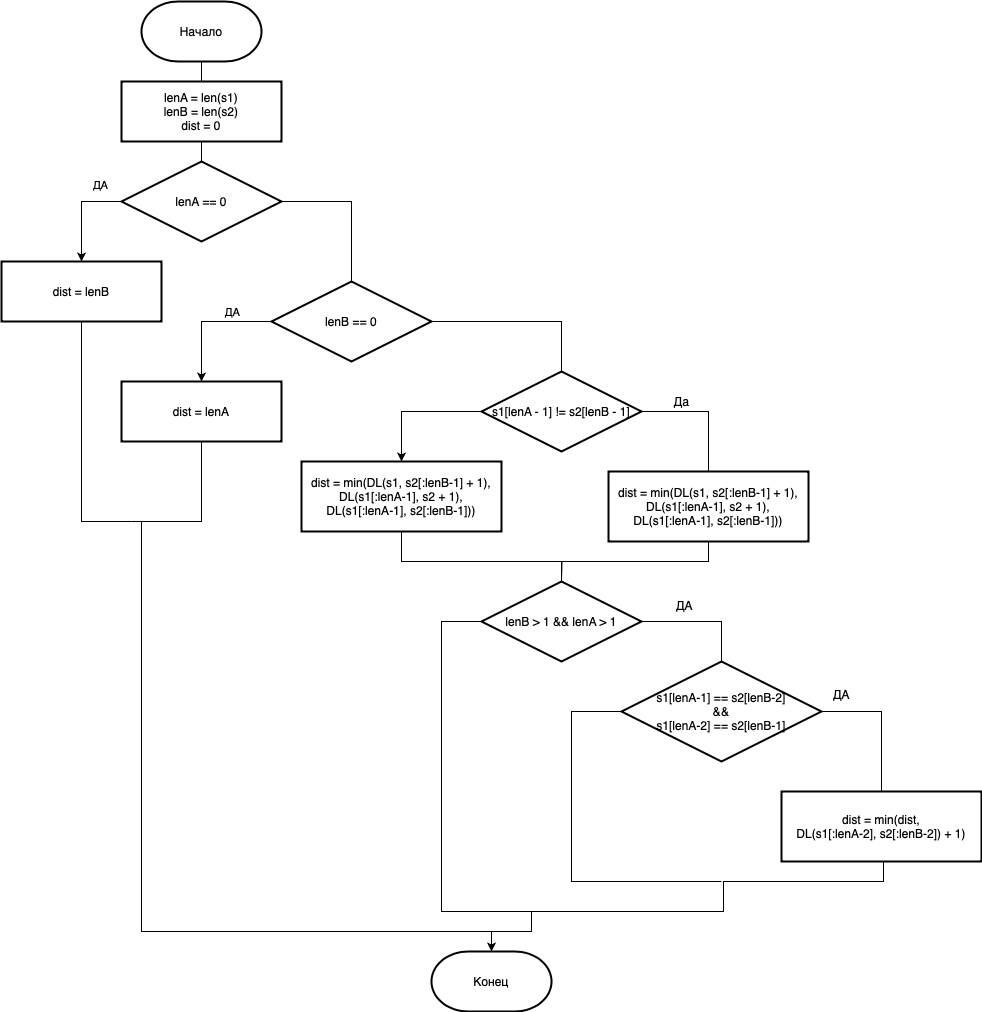
\includegraphics[width=1\linewidth]{img/DLR.png}
	\caption{Схема рекурсивного алгоритма нахождения расстояния Дамерау-Левенштейна}
	\label{fig:mpr}
\end{figure}

\clearpage

\begin{figure}[h]
	\centering
	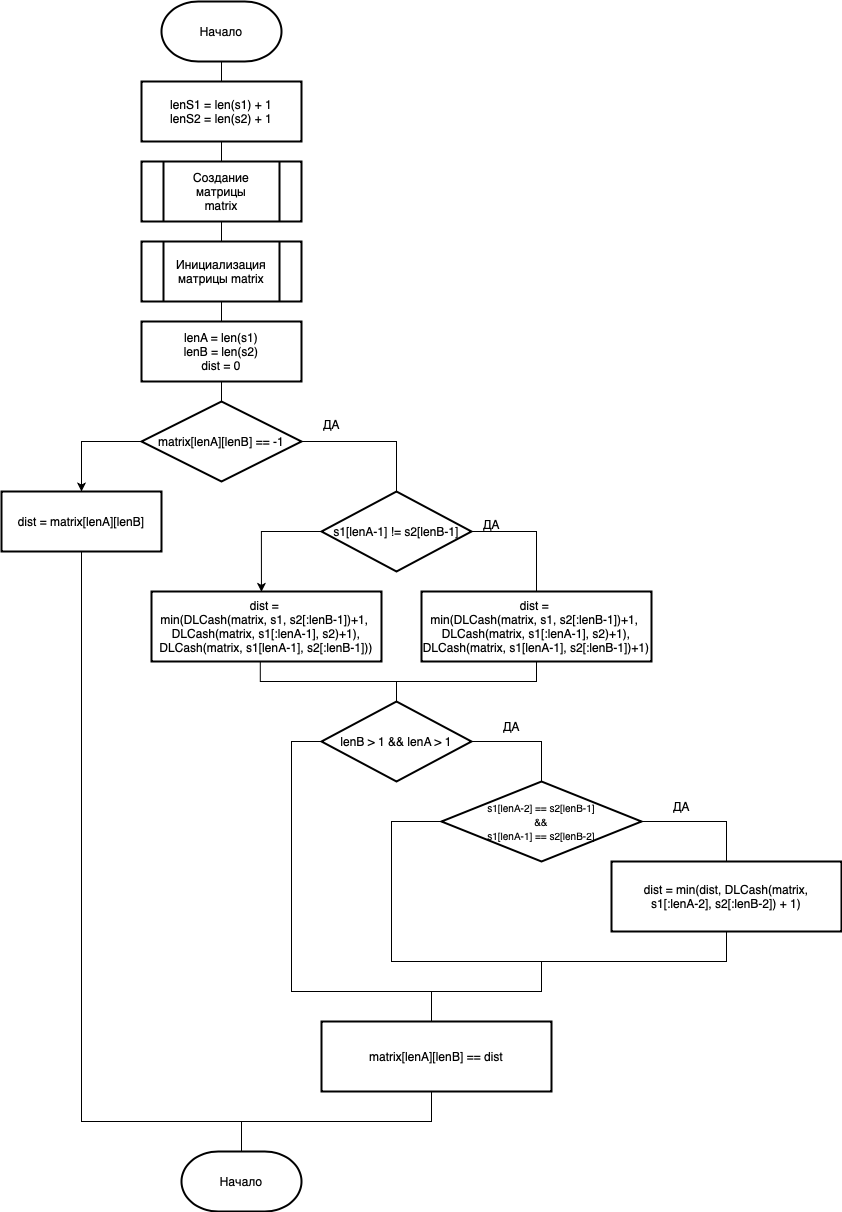
\includegraphics[width=0.8\linewidth]{img/DLC.png}
	\caption{Схема рекурсивного алгоритма нахождения расстояния Дамерау-Левенштейна с кэшированием}
	\label{fig:mpr}
\end{figure}

\clearpage
\section{Требования к ПО}
Требования к программному обеспечению представлены далее:
\begin{enumerate}
	\item На вход подаются две строки в любой раскладке (в том числе и пустые);
	\item ПО должно выводить полученное расстояние.
\end{enumerate}

\section{Вывод}
На основе теоретических даннных, полученных в аналитическом разделе были построены схемы исселедуемых алгоритмов.
